% geometry_and_trigonometry:x07 GDC:YES
\begin{question}
  \hspace*{\fill} [Note Maximale: 7]\par
  \medskip
  \noindent Il y a, au pied d'une colline une tour verticale $TA$ de 36 cm de hauteur. Un chemin rectiligne monte la colline depuis $A$ vers un point $U$. Ces informations sont représentées par la figure suivante.\par
  \medskip
  \begin{center} % or flushleft or flushright
    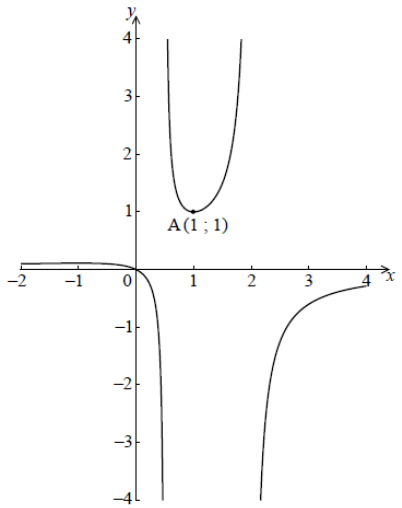
\includegraphics[scale=0.3]{figure_x7}\par
  \end{center} % or flushleft or flushright

  \noindent Le chemin fait un angle de $4^\circ$ avec l'horizontale.\par
  \noindent Le point $U$ sur le chemin est à $25 m$ de la base de la tour.\par
  \noindent Le sommêt de la tour est relié à $U$ par un câble de longueur $x$ (en m).\par
  \begin{enumerate}[label=(\alph*)]
    \item Complétez la figure en représentant clairement les informations ci-dessus.\hspace*{\fill} [3]
    \item Trouvez $x$.\hspace*{\fill} [4]
  \end{enumerate}
\end{question}
